\chapter{Tool Discovery, Routing, and Typed Execution Contracts}\label{ch:C18}

HyperTool's 2026 tool blocks change execution granularity, while selective delegation changes which worker acts and a privilege monitor constrains admissible effects~\cite{du2026hypertool,cui2026unoorchestra,corpus250411703}. These interventions address different boundaries. Their comparison must retain argument validity, dispatch authority, intermediate state, resource accounting, and the distinction between a retrying language-model trace and a repeated external operation.

\section{A tool call is a typed state transition}\label{sec:C18:contract}
A tool exposes a capability through an interface that an agent can invoke. Its scientific description should include input and output types, preconditions, side effects, failure states, authority requirements, and version identity. A natural-language name and argument schema provide only part of that contract. Two tools with identical JSON shapes can have different resource scopes or effect semantics. A model can produce a syntactically valid call that is operationally wrong.

For environment state space $\mathcal X$, argument space $\mathcal U_j$, observation space $\mathcal O_j$ and receipt space $\mathcal E_j$, represent tool $j$ by a transition kernel
\begin{equation}
 \mathcal T_j(dx',do,d\eta\mid x,u,A),
 \quad u\in\mathcal U_j.
\end{equation}
Here $A$ is current trusted authority, $o\in\mathcal O_j$ an observation and $\eta\in\mathcal E_j$ a typed receipt or uncertainty state. Rejection, timeout and partial completion need explicit outcomes; a partially observed kernel does not give the model access to $x$ or to privileged authorization state. A successful HTTP response is not necessarily proof that the intended business effect occurred; a timeout is not proof that it did not. Chapter~\ref{ch:C13} analyzes the resulting recovery ambiguity.

The model's tool-use decision has at least three stages: select a capability, construct its arguments, and decide how to interpret its result. Toolformer and ReAct are foundational examples of learning or prompting tool-augmented behavior~\cite{schick2023toolformer,yao2022react}. They should not be treated as descriptions of every current runtime. Contemporary systems add discovery, typed schemas, external enforcement, code-based composition, and durable execution. Each addition changes the effective policy and its failure surface.

A contract should identify which fields are exact. Resource identifiers, operation keys, and authority scopes should not be reconstructed from a vague summary when exact values are available. Free-text queries can remain flexible. Output records should separate authoritative data from tool-generated explanations and untrusted external content. Returning a page that contains instructions does not grant those instructions authority over the agent. The wrapper must preserve that distinction when the result enters active context.

For evaluation, define success at the tool boundary and at the task boundary. A schema-valid call can fail a tool precondition. A tool-successful call can be irrelevant to the task. A task can appear solved while the agent produces an unauthorized side effect. These outcomes need separate labels. A single ``tool accuracy'' number is ambiguous unless it specifies whether it measures tool selection, argument validity, execution, or complete justified behavior.


\section{Discovery changes the action space}\label{sec:C18:discovery}
Discovery provides the agent or harness with the currently available capabilities. It can involve a static catalog, server-provided schemas, search over tool descriptions, or staged loading of detailed definitions. The catalog is part of the policy's information state. Adding or removing tools changes the represented proposal interface and can alter performance even when the model weights and task distribution remain fixed. Discovery does not itself grant authority: the dispatcher independently restricts which discovered operations may execute.

Large catalogs create both token and discrimination costs. Injecting every complete schema can consume context and expose near-duplicate actions. A two-stage mechanism can retrieve candidate tools using coarse descriptions and load exact schemas only before invocation. This reduces active input but can exclude the necessary tool at the discovery stage. Evaluation should report catalog recall separately from correct use among discovered candidates. An oracle candidate list is a diagnostic condition, not an executable baseline.

Tool descriptions are themselves data that can be stale, misleading, or adversarial. A server can expose a harmless-looking title while its implementation has broader effects. A retrieved description can include instructions unrelated to the capability. Treating the description as an authoritative system instruction expands the trust boundary. Metadata can guide selection without being allowed to redefine the user's task or authority.

Current MCP separates discovery and invocation through its tool feature and schemas~\cite{mcp2026tools}. A capability catalog can vary with per-request authorization, so a cached list should be associated with the authorization context that produced it. The detailed protocol semantics are developed in Chapter~\ref{ch:C19}. The application-level consequence is that catalog identity, credential scope, and schema version belong in the decision record. A tool visible to one principal need not be visible to another.

Discovery can also create a training-deployment mismatch. A policy trained with a fixed tool ordering can exploit names or positions rather than robust semantic selection. At deployment, reordered or expanded catalogs can degrade selection. Controlled tests should permute catalog order, introduce unrelated near-name tools, and hold schema content constant. A model that fails these tests may have learned a brittle interface shortcut rather than a transferable tool-selection mechanism.

The proposed implementation caches catalogs with explicit expiration and invalidation, stores a schema digest per selected tool, and validates the exact schema again before dispatch where required. It distinguishes a missing capability from an unavailable credential and from a temporary execution failure. Those errors lead to different next actions: revise the plan, request an authorized scope change, or retry under a bounded recovery policy.


\section{Routing as constrained resource allocation}\label{sec:C18:routing}
A router chooses among direct answering, tool execution, retrieval, specialized models, and delegated workers. Its objective should combine task value, latency, cost, and authority rather than maximizing a tool-use rate. Calling a tool unnecessarily can introduce expense and risk; refusing a necessary tool can create an unsupported answer. Tool abstention and tool invocation are both decisions requiring calibration.

Let $j$ index a finite catalog of admissible routes and let $Q_j(s)$ estimate expected task utility in state $s$. Let $C_j(s)$ and $L_j(s)$ estimate resource cost and latency, with nonnegative conversion weights $\lambda_c$ and $\lambda_l$. A proposed decision rule is
\begin{equation}
 \widehat j(s)\in\arg\max_{j\in\mathcal J_A(s)}
 \{Q_j(s)-\lambda_c C_j(s)-\lambda_l L_j(s)\},
\end{equation}
where $\mathcal J_A(s)$ contains the authority-permitted routes and an explicit no-effect route $j=0$. The latter permits abstention or a request for missing information, so the maximization remains defined when no effectful route is allowed. Ties require a declared selection rule. The estimates depend on model version, tool reliability, queueing, and remaining budget. Optimizing a router on static average prices can be inappropriate when latency or tool availability changes. Constraints should be enforced before ranking, rather than represented only as a large penalty that the model may trade away.

The estimated objective also needs an uncertainty boundary. Write $v_j$ for the true expected net utility under one fixed configuration and $\widehat v_j$ for the estimate used by the router. If simultaneous bounds $|\widehat v_j-v_j|\leq b_j$ hold for every feasible route, then, for $j^\star\in\arg\max_jv_j$ and $\widehat j\in\arg\max_j\widehat v_j$,
\begin{equation}
 v_{j^\star}-v_{\widehat j}
 \leq b_{j^\star}+b_{\widehat j}
 \leq2\max_j b_j.
\end{equation}
Insert and subtract the two estimates; the estimated-utility difference is nonpositive by selection. This conditional deduction needs simultaneous coverage, not a separate nominal interval interpreted after inspecting every route. It also assumes a correct current feasible set. Smaller utility uncertainty cannot repair a stale grant, an unmodeled side effect, or support missing from the route logs. Reusing estimates after a model, memory bank or worker interface changes requires a new compatibility argument.

If $L_j$ is mean latency, this rule does not enforce a deadline guarantee. For random completion time $D_j$ and deadline $d$, a tail-aware feasible set can additionally require
\begin{equation}
 \mathcal J_{A,d,\alpha}(s)=
 \{j\in\mathcal J_A(s):P(D_j>d\mid s)\leq\alpha\},
 \qquad \alpha\in[0,1].
\end{equation}
The probability must include queueing, tool retries, and validation under the intended offered load. Two routes can have identical means and different deadline-miss probabilities. Estimating a low-probability tail from a small successful-call sample is insufficient, and timed-out calls remain in the distribution. If every useful route violates the constraint, the system must expose infeasibility or choose a declared degraded mode; replacing the empty set with an unqualified fast answer would change the requirement.

Uno-Orchestra jointly emits task decomposition and admissible model-primitive assignments rather than using an independent decomposition stage followed by a fixed dispatcher~\cite{cui2026unoorchestra}. Its training uses verified worker interactions and a multi-turn objective with intermediate feedback. This is a learned orchestration policy, not evidence that every tool should be delegated. Its benchmark aggregation, worker pool, verifier, and cost boundary determine the meaning of its reported efficiency.

A router's confidence should be evaluated against route-specific outcomes. A model can be confident that a tool is relevant while being uncertain whether its argument values are correct. A worker can solve a subtask but return evidence in an unusable format. Treat route selection, execution, and integration as separate stages. A failed integrated result should not automatically label the route itself wrong if the downstream merger discarded a valid answer.

Training data for routing can be censored. Logs contain outcomes only for routes actually chosen; the unchosen alternative's success is unknown. Supervised imitation of historical routes can reproduce a prior system's biases. Counterfactual evaluation requires randomized exploration where appropriate, controlled replay, or justified off-policy assumptions. Chapter~\ref{ch:C17} explains why missing support and changed conditioning limit importance-weight interpretations.

The proposed baseline set includes a strong single route, a deterministic rule router, a cost-only router, and a learned utility router. Match complete budgets and retain unsuccessful calls. A router that improves average success by using more expensive workers has a useful capability result but has not established equal-budget efficiency. A Pareto comparison is often more informative than a single weighted score.


\section{Argument construction and result validation}\label{sec:C18:arguments}
Argument generation translates a task and its evidence into an executable object. The model must identify entities, select current values, satisfy cross-field constraints, and preserve exact strings where required. JSON syntax is the easiest part of this problem. A call can satisfy a schema while naming the wrong account, using a stale resource version, or combining fields that are individually valid but jointly inconsistent.

Use layered validation. The parser checks serialization. The schema checks types and required fields. The application checks domain preconditions and cross-field constraints. The authority monitor checks whether the operation is permitted. The remote service checks its current state. These layers should return distinguishable errors so the agent can repair the responsible field without broad speculative retries. A generic failure message can induce repeated changes to already correct arguments.

Constrained decoding can reduce malformed outputs by restricting token sequences to an allowed language. It does not establish that the selected entity or action is correct. It can also alter the behavior distribution used for training and likelihood accounting. If a rollout applies schema constraints, record them with the sampled output rather than recomputing probabilities under an unconstrained model. Syntactic reliability and statistical consistency interact at this interface.

Result validation likewise needs several levels. A parser can confirm that a returned object matches the declared type. A tool-specific validator can check a checksum, resource version, or test result. Semantic interpretation decides what the observation implies for the task. A language-model explanation generated by the tool is not automatically independent verification of the same model's action. Preserve raw evidence when it is needed to audit that inference.

One proposed argument-provenance record maps each consequential field to its source: direct user input, retrieved evidence, deterministic transformation, or model inference. This can be lightweight for read-only search queries and stricter for effects. If an identifier comes from an untrusted document rather than the authorized workspace, the dispatcher can detect the difference. The record does not make inferred values correct, but it makes their basis reviewable.

Evaluation should include near-valid errors. Test correct schemas with wrong identifiers, stale versions, units, boundary values, and conflicting fields. Include tools whose names are similar but whose effects differ. A benchmark containing only malformed JSON can overstate practical tool competence because it ignores the harder grounding problem. Conversely, a benchmark that scores only final task success can hide a substantial improvement in syntax while another subsystem remains the bottleneck.



Figure~\ref{fig:C18:overview} isolates the mechanism and its stated information boundaries.
\begin{figure}[!htbp]
\centering
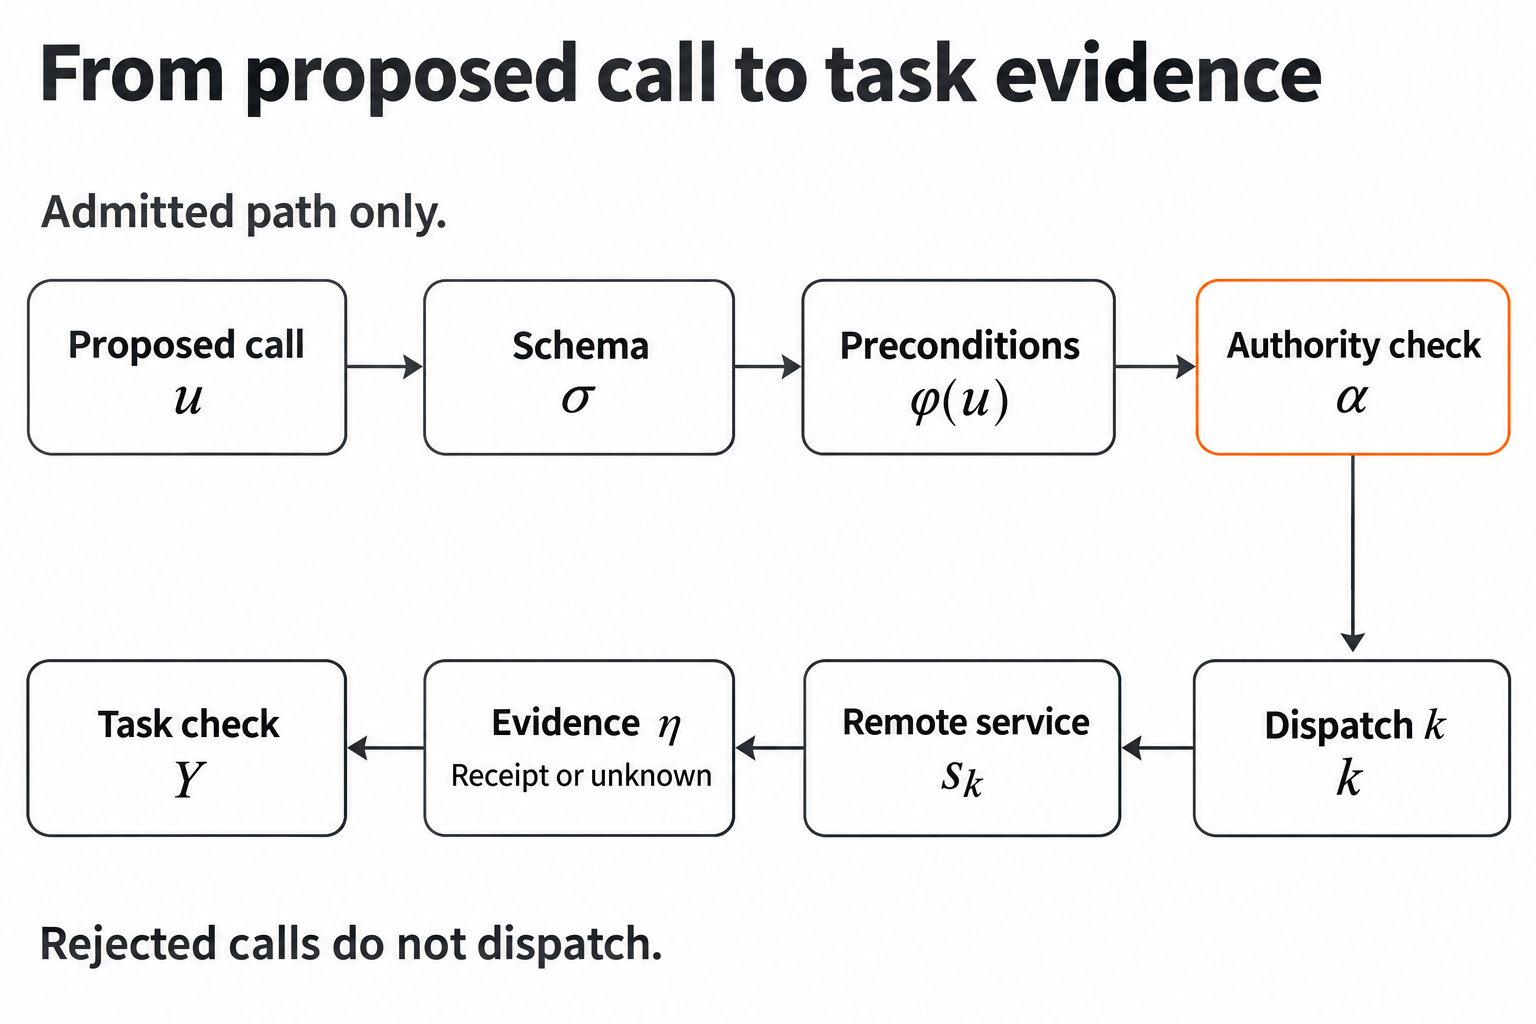
\includegraphics[width=\linewidth]{book/figures/assets/F18review.png}
\caption{A normative admitted tool path: schema, domain and current-authority checks precede dispatch. Here $\alpha$ denotes the authority epoch. Actual service evidence $\eta$, including unresolved outcomes, is recorded separately from a task check $Y$. This schematic does not claim that framework defaults enforce every boundary, that admission and remote commit are atomic, or that a receipt proves task correctness. Figure-local $\sigma$ names the schema, $\varphi(u)$ a domain predicate, $k$ the logical operation identifier, and $s_k$ its servicing endpoint.}
\label{fig:C18:overview}
\end{figure}

\section{Execution granularity and local programs}\label{sec:C18:granularity}
One model decision per atomic tool call exposes every intermediate value to the main reasoning trace. This can be useful when each observation changes the plan, but wasteful when several operations form a locally deterministic subroutine. Code-based composition can keep temporary values inside an execution environment and return only the result needed by the outer policy. It changes execution granularity, not merely trace compression.

HyperTool uses an executable block that can call existing tools through their schemas and manipulate intermediate values locally~\cite{du2026hypertool}. Its method couples that interface with synthesized and verified training trajectories. The reported gains therefore involve both a new action abstraction and training for its use. A comparison that gives only one condition the specialized training cannot attribute the full result to block execution alone. The public paper now permits a method-level assessment beyond an abstract-only lead, while independent reproduction remains unestablished here.

The mathematical distinction is between choosing a sequence of atomic actions with model feedback at every step and choosing a program $p$ whose internal transition sequence is executed under a runtime. A program can express loops, branches, and dataflow compactly. Its correctness requires both valid tool calls and correct control flow. It can reduce model-call latency while making intermediate effects less visible to the outer policy. The tradeoff depends on how often new observations should trigger reconsideration.

A constructed example retrieves two coordinates and computes a distance. If geocoding and arithmetic are deterministic under the request, one block can pass values locally without asking the model to copy them between calls. If the first geocoding result is ambiguous, the block should expose that ambiguity or apply a declared rule rather than silently choosing a location. Grouping does not eliminate the need for checkpoints at semantically meaningful uncertainty boundaries.

Security enforcement must cover calls inside the block. Wrapping the outer executable tool while allowing unrestricted internal tool access can bypass per-tool policy. Every consequential internal invocation should preserve the principal, authority, operation identity, and audit trail. A returned concise result should retain references to the internal effect receipts. Context savings should not be purchased by deleting the evidence needed for recovery.

The proposed ablation compares atomic calls, an untrained block interface, and a block-trained policy under matched models and budgets. Measure model tokens, internal tool calls, critical-path latency, error recovery, and hidden effects. A reduction in outer calls is informative but incomplete. The relevant question is whether the new granularity preserves justified task behavior while reducing complete execution cost.


\section{Retry pruning and failure memory}\label{sec:C18:pruning}
Tool failures create a sequence of attempted repairs that can dominate an agent's context. Some failures are transient; others reveal a wrong assumption or an invalid action. Repeating the same call can be appropriate for a rate limit and inappropriate for a permission denial. A retry policy should classify the failure before deciding whether to repeat, revise, replan, or stop.

PruneTIR distinguishes successful error resolution, a stuck repair trajectory, and repeated failures that justify temporary tool suspension~\cite{zhang2026prunetir}. It prunes resolved error traces, can resample from an earlier state, and can stop further tool use after retry conditions. Its primary reasoning evidence is concentrated in tool-integrated tasks such as mathematics. The observed correlation between erroneous calls and wrong answers does not by itself prove that deleting errors causes correctness; the interventions and ablations supply the relevant additional evidence.

Pruning has a semantic cost. A resolved error can contain a negative lesson needed to prevent recurrence. Removing the detailed trace from active context can be reasonable while preserving an explicit failure state or procedural warning outside it. Conversely, retaining every stack trace can bias the model toward a failed approach. The controller should distinguish temporary execution noise from evidence that invalidates the current plan.

Resampling from an earlier state is safe only when the environment is also restored or when the removed actions had no relevant effects. Rewinding the conversation does not rewind an external service. If a failed-looking operation partially committed, retrying an alternative can create inconsistent state. A tool-pruning method evaluated in a controlled interpreter should not automatically be generalized to irreversible workflows. State restoration and effect reconciliation belong in the deployment contract.

A proposed failure memory stores error class, attempted action, relevant state version, repair outcome, and conditions under which retry became valid. It should avoid turning an environment-specific failure into a global tool prohibition. If the tool version changes, old failures may become obsolete. This connects retry control to procedural memory and temporal validity rather than treating it as a token-removal heuristic.

Testing should retain both benign transient failures and persistent semantic failures. Compare unbounded retries, fixed retry limits, typed retry rules, and learned failure-aware control. Measure completion, wasted calls, duplicated effects, recurrence of the same error, and premature abandonment. A method that reduces calls by refusing difficult tasks needs to be distinguished from one that reaches the same success rate more efficiently. All failures and abstentions remain in the denominator.


\section{Privilege control at the dispatch boundary}\label{sec:C18:privilege}
Progent's concrete mechanism is a policy over tool names and argument values, checked before execution~\cite{corpus250411703}. A model can propose an initial policy or an update, but deterministic analysis distinguishes a narrowing from an expansion. An expansion requires an authorized approval path under the paper's design. This is stronger than asking the same model to reconsider whether its own call is safe, because enforcement is external to the action-generating policy.

Let $P$ denote an allowed-call set and let $P'$ be a proposed update. A monotonic-confinement check asks whether $P'\subseteq P$. Under complete mediation and faithful policy interpretation, automatically accepting only such updates prevents unapproved expansion through that path. It does not establish that $P$ was initially minimal, that an allowed call is semantically correct, or that all external effects pass through the monitor. Those assumptions determine the guarantee's scope.

Schema-based constraints can express useful restrictions on resource identifiers, recipients, or operation types. They can also be too coarse. A call can satisfy a permitted path pattern while reaching a resource through an alias or redirection whose semantics the monitor does not model. A broad code-execution tool can hide many effects behind one allowed argument string. The policy language and tool wrapper must jointly model the effects being controlled; otherwise the apparent boundary can be incomplete.

Utility and security should be measured together. A policy that blocks every call achieves a trivial form of attack prevention while failing legitimate tasks. A permissive policy can complete tasks while leaving unnecessary authority open. Evaluate benign completion, prohibited-call rejection, false blocks, and unexercised excess privilege where the threat model requires it. Attack-success scores alone do not measure the entire allowed action surface.

Memory and discovery influence this boundary. A retrieved skill may propose a new tool or broader scope, and an updated catalog may expose a capability the initial policy did not include. The system should treat that as an explicit authority question rather than silently inheriting the new capability. The model can explain why an expansion would help; it should not be able to grant the expansion merely by rewriting its context.

The practical architecture places the check immediately before dispatch, with the current applicable policy and validated arguments. Earlier checks can support planning but do not cover intervening corrections. Record a receipt tying the executed call to the policy version that admitted it. This provides the causal link needed to audit whether a later undesirable effect came from policy design, stale authority, wrapper bypass, or incorrect tool behavior.

The inspected Progent implementation exposes this boundary through \path{check_tool_call} and wrappers in its \texttt{secagent.tool} module. Policy type checking is separate from containment analysis. In \path{security_policy_subset_check}, the generated-policy entries are compared through schema constraints, and an unproved containment result is rejected rather than assumed safe~\cite{repo_progent2026}. The source observation is narrower than a proof of the complete deployed system: it concerns the represented policy subset and the solver translation at that revision. Wrapper coverage, service effects, and manually configured policy semantics still require separate validation.

The configuration is part of this claim. At the inspected revision, \path{check_tool_call} warns and returns when no security policy is initialized; generated-policy containment is enabled only when \path{SECAGENT_ONLY_ALLOW_NARROW} is true, whose code default is false. The \path{tool.py} type-check wrapper does not call the separate checking helper, and that helper returns warnings~\cite{repo_progent2026}. The existence of these functions therefore does not prove that every deployment enables confinement or rejects a malformed policy. A conformance test must bind initialization, configuration, wrapper coverage and rejection behavior before measuring benign utility or attack resistance. These source observations do not assert that the paper's evaluated configurations used the defaults.

The logical test can be expressed as searching for an argument value $x$ satisfying $P_{\mathrm{new}}(x)\land\neg P_{\mathrm{old}}(x)$. A satisfying assignment is a counterexample to narrowing. If a represented old policy allows an amount at most 100 and the proposed policy allows an amount at most 200, $x=150$ witnesses expansion. If the new bound is 50, the corresponding formula is unsatisfiable under ordinary numeric semantics. These numbers are an analytic illustration, not a benchmark result. The validity of the conclusion depends on whether the schema-to-solver translation faithfully captures the argument and tool semantics.

The type checker also matters because a policy restriction on an argument absent from the actual tool schema can be meaningless or malformed. Validation should reject that mismatch before enforcement, rather than allowing a generated policy to create the appearance of confinement. Conversely, a schema-valid restriction can still be inadequate if the tool accepts aliases, resolves paths, or performs downstream operations outside the modeled field. Syntactic alignment closes one failure mode without closing every semantic bypass.

For an implementation study, instrument policy generation, type-check outcome, containment outcome, admitted arguments, and the wrapped function that ultimately executes. Include solver-unknown or translation-failure cases and verify that they cannot silently broaden policy. Compare the monitor's decision with an independently specified small reference action set on synthetic tools whose semantics are known. Then test realistic wrappers to determine whether all consequential paths are mediated. This is a proposed test sequence; no additional security measurements are asserted here.


\section{A tool-use experiment that can falsify the mechanism}\label{sec:C18:evaluation}
A strong tool study defines comparison axes before ranking methods. For selection, measure whether the necessary capability is discovered and chosen. For arguments, measure structural and semantic validity. For execution, measure preconditions and effects. For integration, measure whether the result changes the task state correctly. For authority, measure whether the call is permitted. Aggregating these into one score can be useful for a product decision, but the component outcomes are needed for scientific explanation.

The proposed baseline cohort keeps the underlying model and tools fixed while varying catalog presentation, routing policy, validation, and execution granularity. Include a direct single-agent baseline, a deterministic router, a learned router, and an oracle tool-selection condition for diagnosis. When specialized training is added, report it as a separate factor rather than silently comparing a trained interface against an untrained one. Count all controller, verifier, worker, and retry calls.

Task construction should include impossible requests, missing permissions, changed schemas, ambiguous entities, and tools that return plausible but stale data. A competent agent should sometimes abstain or request information. A benchmark in which every task is solvable with one known tool can reward overconfident invocation. Negative cases are necessary to measure whether the policy understands applicability and authority rather than simply matching names.

Contamination controls include tool-description overlap, released task trajectories, and environment fixtures. Training on one tool's examples can transfer useful syntax while leaking benchmark-specific workflows. Separate unseen schemas, unseen compositions, and unseen environment states. A model that handles a renamed familiar tool has achieved a different generalization target from one that composes new capabilities under a changed state distribution.

Latency and cost should include discovery, schema loading, validation, local program execution, remote calls, retries, and reconciliation. Report task-level distributions and overload behavior when concurrency matters. A block interface can reduce model transitions while increasing internal tool work; a router can improve success by choosing slower workers. Neither is intrinsically better without a workload and service objective.

The reviewed methods establish concrete design choices: learned selective delegation, inference-time repair pruning, executable local composition, and external privilege enforcement. Their mechanisms address different bottlenecks. A combined system is a hypothesis whose interactions must be evaluated, particularly where context editing changes routing evidence or where a composed block changes the enforcement surface. The next chapter treats the protocol layer that carries these tools and delegated tasks across process boundaries.

